%% Setup Document
\documentclass[]{article}
\usepackage[danish]{babel}
\usepackage[utf8]{inputenc}
\usepackage[margin=2.5cm]{geometry}
\renewcommand{\baselinestretch}{1.5}
\usepackage{pdfpages}
%% Setup Section Counters
\setcounter{secnumdepth}{2}
\setcounter{tocdepth}{2}
%% SetUp Figures
\usepackage{graphicx}
\graphicspath{ {Figures/} }
\usepackage{caption}
\usepackage{subcaption}
\usepackage{geometry}
\usepackage{subfiles}
%% Update Enumerate to make Use Cases possible 
\usepackage{enumerate}
\usepackage{enumitem}
%% Enable figure wrapedin text
\usepackage{wrapfig}
%% Change Subsubsection spacing
\usepackage{titlesec}
\titlespacing*{\subsubsection}{0pt}{0.4\baselineskip}{0pt}
%% Unknow
\usepackage{amsmath}
\usepackage{gensymb}
\usepackage{appendix}
\usepackage{float}
\usepackage{textcomp}
\usepackage{lastpage}
\usepackage[T1]{fontenc}
\usepackage{lmodern}
\usepackage{cite}


%% Setup frontpage
\newcommand*{\titleGP}{\begingroup 
	\renewcommand{\baselinestretch}{1} 
	\begin{picture}(0, 0) (-390,31)
	\includegraphics[width=0.12\textwidth]{logo1.png}
	\end{picture}

	\centering 
	\vspace*{\baselineskip} 
	
	\rule{\textwidth}{1.6pt}\vspace*{-\baselineskip}\vspace*{2pt} % Thick horizontal line
	\rule{\textwidth}{0.4pt}\\[\baselineskip] % Thin horizontal line
	
	{\LARGE Eksamen\\  [0.3\baselineskip]
		 Holdnummer C6} \\[0.2\baselineskip] % Title
		 %De sejeste mennesker : Caféen?}\\[0.2\baselineskip] % Title
	
	\rule{\textwidth}{0.4pt}\vspace*{-\baselineskip}\vspace{3.2pt} % Thin horizontal line
	\rule{\textwidth}{1.6pt}\\[\baselineskip] % Thick horizontal line
	
%	\scshape % Small caps
%	Sidste øjekast på applikationen \\
	
	
%	\vspace*{2\baselineskip} % Whitespace between location/year and editors
	
	af \\[\baselineskip]
    {\Large  Camilla Ejsing (smb912@alumni.ku.dk) \\ \left( Nicolai Manique (jpm235@alumni.ku.dk) \& \\ Søren L. Nissen (rhc148@alumni.ku.dk) \right)    \par} % Editor list
%	{\Large  Camilla Ejsing \\ Mohammed Sami Elnono \\ Nicolai Manique \& \\ Søren L. Nissen    \par} % Editor list
    {Instruktorer: Alexander Winther Uldall \& \\ (Sven Uhrenholdt Frenzel) \par }
    {GitHub-arkiv: https://github.com/cejsing/Softwareudvikling \par}

%    {Gammelt GitHub-arkiv: https://github.com/samielnono/Project-Cafeen \\
%    Nyt GitHub-arkiv: https://github.com/SNissen/ProjectCafeenC6 \par}
	{\itshape Datalogi : Softwareudvikling \par} % Editor affiliation
	
	\vfill % Whitespace between editor names and publisher logo
%	\includegraphics[height=0.4\textheight]{FrontPage.jpg}
	\vfill
	{\scshape 2016} \\[0.3\baselineskip] % Year published
	{\large }\par % Publisher
	
\endgroup}

\begin{document}

\thispagestyle{empty} % Removes page items
%\titleGP % This command includes the title page
\pagebreak

\pagenumbering{roman} 
\tableofcontents
\newpage

\pagenumbering{arabic}

\section{Projektbeskrivelse} \label{Projektbeskrivelse}
% En kort beskrivelse af jeres applikation og dens anvendelse. Væsentlige tolkninger af opgaveteksten, hvor I fandt den tvetydig, og afgrænsninger I har valgt at foretage skal beskrives og begrundes.
I denne rapport vil udviklingen af et nyt lageroptællingssystem til studiebaren Caféen? på Science, Københavns Universitet blive gennemgået. \\
Lageroptællingssystemet skal være brugervenligt, simpelt at bruge ved både åbning og lukning. \\
Til denne opgave har jeg haft adgang til tidligere produceret kode, skabt netop til Caféen? med selv samme formål. Jeg har haft 3 uger til at sætte mig ind i og videreudvikle på denne kode, hvor jeg har lagt vægt på at videreudvikle frontend og klargøre lageroptællingssystemet til brug på Caféen?. \\ \\

Grundet den korte tid til at videreudvikle på projektet, har jeg besluttet at gøre mine iterationer meget korte, og sætte forventningerne derefter. Da iterationer iflg. agile ?? normalt er 2-3 uger pr. iteration, ville jeg kun kunne nå en enkelt iteration. Derfor har jeg valgt at lave iterationer a en uges varighed, og jeg kan derfor nå 3 iterationer, hvortil jeg laver user stories og use cases. \\ \\
I den første iteration bruges der meget tid på at jeg skal sætte mig ind i den iforvejen eksisterende kode, således der kan videreudvikles og laves eventuelle rettelser og forbedringer. \\
Sørge for at flere brugere kan tilgå systemet og relevant historik gemmes, frontenden gøres simpel og let at bruge, overskuelighed. \\
Bruge tid på at se koden igennem for fejl, mangler, gentagelser. \\ \\

Sammen med min gruppe udviklede jeg et nyt lageroptællingssystem til Caféen?. \\
Vi lagde vægt på simplicitet i backenden, da der i beskrivelsen af opgaven blev lagt vægt på at koden skulle være simpel og let at ændre. \\
Applikationen er kodet sådan, at backenden indeholder funktioner, der kan håndtere forskellige problemer, og frontenden eksekverer så disse funktioner på fornuftig vis. Dette gør det nemt for en anden programmør at sætte sig ind i hvordan koden fungere, og ønsker man at tilføje en funktion kan man blot udbygge den nuværende kode. Dette gør programmet yderst fleksibelt og nemt at gå til. Ud over dette var der også et ønske om at kunne håndtere forskellige varegrupper og begivenheder med forskellige priser. Dette var noget af det første vi kastede os over, og det har været vores fokus at få disse tre ting til at fungere. Ud over dette har historikken været noget der i opgavebeskrivelsen var lagt vægt på historikken. At man kunne gå tilbage i tiden og se ændringer, eller rettere, ændringer skulle ikke gælde bagud. Vi har valgt at lægge fokus på at kunne følge ændringernes gang. Dette kan der læses mere om koden afsnittet "Design". Alt i alt kan man opsummere vores fokus punkter til: 
\begin{enumerate}
	\item \textbf{Simpel backend} \\ Skal være til at overskue hvor ting ligger.
	\item \textbf{Nemt at ændre} \\ Skal ikke være et låst program, det skal kunne viderusvikles.
	\item \textbf{Brugbart udgangspunkt} \\ Vare, varegrupper og begivenheder klar til brug.
	\item \textbf{Simpel håndtering af historik} \\ Skal ikke forstyrre funktionen af resten af programmet, og skal være nemt at tilgå. 
\end{enumerate}
Det har i projektbeskrivelsen været lidt tvetydigt hvorvidt man ønskede at alle varer i samme gruppe \textit{skulle} have samme pris, eller om dette var en procedure man havde nu, men ønskede at ændre. Da vi har haft fokus på at vores program skulle være fleksibelt har vi valgt at lægge fokus på fleksibiliteten, og har dermed givet hver enkelt vare sin egen pris. Men har så også gjort sådan at man kan tilføje prisændringer for hele varegrupper. En specifik problemstilling vi har haft store problemer med at håndtere har været håndteringen af sprut. Det har fra Cafeén?s side været udtrykt, at man ønskede at opgøre sprut i vægt, men det har været svært at finde ud af præcis hvordan de ønskede denne problemstilling håndteret. Se \ref{Sprut} for nærmere beskrivelse af løsningen på denne problemstilling. 
\pagebreak[3]

\section{Krav} \label{Krav}
I projektets begyndelse kom kunderepræsentanten Jenny (fra Caféen?), som klargjorde behovene til et nyt lagerstyringssystem i forbindelse med optællinger på studiebaren Caféen?, som er drevet af frivillige studerende. Det blev gjort klart, at lagerstyringssystemet skal kunne håndtere varegrupper, varer og kunne registrere hvilken type begivenhed, der har været forud for optællingen. Sådan en begivenhed kunne eksempelvis være, at der er åbent på hverdage eller at Caféen? er udlejet på en lørdag. Derudover nævntes et fremtidigt behov for et regnskabssystem i forbindelse med lagerstyringen, som de udvidede specifikationer for systemet lægger sig op ad. \\
Vi noterede følgende punkter om lagerstyringssystemet under mødet med repræsentanten:
\begin{enumerate}
	\setlength{\itemsep}{-3pt}
	\item Det skal være simpelt
	\item Det skal være webbaseret
	\item Det skal være neutralt
	\item Det skal ikke indeholde fancy features
	\item Man ønsker at håndtere varegrupper og varer
	\label{databaseOne}
	\item Man ønsker at kunne angive antal varer
	\item Man ønsker at kunne ændre navne og oplysninger på varer og varegrupper
	\item Man ønsker at have forskellige prissatser baseret på typer af arrangementer
	\item Man ønsker at kunne slette varer
	\label{databasetwo}
	\item Man ønsker at kunne se tidligere varer og priser på varer
	\item Historikken må ikke kunne påvirkes af senere vareændringer
	\item Systemet skal kunne håndteres af ikke-dataloger
	\item Systemet skal kunne håndtere flere brugere på en gang.
\end{enumerate}
\noindent Det blev afklaret af kunden, at historik ikke kan opdateres samtidig med salg af varer, da disse ikke bliver registreret af et kasseapparat. Det er derfor nødvendigt, at historikken håndteres som en del af optællingen sidst på dagen. \\
\noindent Efter mødet vurderede vi, at punkt \ref{databaseOne} til \ref{databasetwo} kan håndteres af en database uden at komme i karambolage med de to sidste punkter. En database vil ikke have nemt ved at håndtere historikken direkte, men dette kan løses ved at alle ændringer i databasen bliver registreret, så brugeren kan få adgang til tidligere stadier (punkt 6). \\
\indent For første release medio juni forventes det, at brugeren kan tilføje en vare til systemet med valgt varegruppe og pris. Det forventes at brugeren kan åbne og lukke en vagt med optællinger som korrekt videregår til databasen over varer. Det forventes derudover at en yderligere udvikling nemt kan understøtte yderligere funktionaliteter i henhold til brugerens oplyste behov. \\
\indent I henhold til brugerens ønsker vil fokus primært være udvikling af backend/database. Databasen vil blive implementeret med tabeller og relationer i forhold til udviklet design og backend vil blive udviklet med fokus på at manipulere databasen på en måde, der passer til kundens krav.

\subsection{User stories}

Ud fra disse overvejelser har vi opstillet følgende \ref{UserStories} user stories:
\begin{enumerate}
	\setlength{\itemsep}{-3pt}
	\item Tilføj vare 
	\item Tilføj varegruppe
	\item Tilføj vare under varegruppe
	\item Ændr prisen på en vare fremadrettet
	\item Ændr information om vare
	\item Lageroptælling ved åbning
	\item Lageroptælling ved lukning
	\item Håndtering af vægt af sprut
	\item Vælg en prisliste (begivenhedtype)
	\item Slet vare i systemet
	\item Foretag varemodtagelse
	\item Der optælles på en seddel og senere vil denne optælling blive skrevet ind
	\item Ændr priserne på alle varer i en varegruppe
	\item Opret en særlig type begivenhed med særlige priser
	\item Tilføj kommentar til optælling
	\item Kasserer vil gerne kunne opholde sidste års indtægter og udgifter i et regnskab
	\item Identificér optæller
	\item Flere skal kunne ændre samtidig
	\item Merge varer
	\item Vis komplet vareliste
	\item Printe grafer over forskellige salgs-/prisudviklinger
	\label{UserStories}
\end{enumerate}
Disse \ref{UserStories} user stories opskrev vi i prioriteret rækkefølge i begyndelsen af projektet. Vi vurderede, at vi som minimum ville kunne nå at implementere de 14 øverste i løbet af hele projektet. Dette vurderede vi ud fra, at vi ville fokusere på overordnede funktionalitet af programmet frem for at fokusere på test af særtilfælde. Derudover besluttede vi at fokusere på en simpel struktur af programmet. \\
Dette betyder, at hvis der på Caféen? eksempelvis først er begivenheden 'almindeligt salg' og senere 'rengøringsdag', og at der ikke er en optælling imellem begivenhederne, som skrives ind, vil denne overgang fra en begivenhed til en anden ikke vil behandlet af systemet, da et sådant specialtilfælde vil udvide kompleksiteten. \\
Hvorvidt disse krav blev nået, prioriteringen og implementering af kravene vil blive diskuteret i afsnit \ref{Diskussion}.

\subsection{Use cases}

Ud fra vores \ref{UserStories} user stories har vi i løbet af projektet opstillet 14 use cases for nogle af vores user stories.
\begin{enumerate} [label= \# \arabic*:]
	\item  \textbf{Tilføj vare til systemet.} \\For at en varetilførsel skal kunne gå igennem, skal brugeren have noteret navnet på varen samt dens standardpris (og varegruppe). Brugeren vil se felter for disse oplysninger samt en “gem”-knap. Ved tryk på gem vil det tjekkes om data er indtastet korrekt. Oplysningerne vil ved korrekt indtastning indskrives i databasen for de relevante tabeller.
	\item \textbf{Tilføj varegruppe} \\En varegruppe skal have et navn for at kunne gå igennem. Brugeren vil se felter for disse oplysninger samt en “gem”-knap. Ved tryk på gem vil det tjekkes om data er indtastet korrekt. Oplysningerne vil ved korrekt indtastning indskrives i databasen for de relevante tabeller.
	\item \textbf{Tilføj vare til varegruppe.}\\Varen og varegruppen skal allerede eksistere for at man kan associere dem. Brugeren vil have flere muligheder for at kunne lave denne association. Oplysningerne vil ved korrekt indtastning indskrives i databasen for de relevante tabeller.
	\item \textbf{Ændre priser på en vare fremadrettet}\\Varen skal eksistere. Brugeren vil kunne se en række priser for varen afhængigt af begivenhedstypen. For hvert felt kan brugeren ændre prisen og derefter trykke gem. Oplysningerne vil ved korrekt indtastning indskrives i databasen for de relevante tabeller.
	\item \textbf{Ændre information om vare}\\Varen skal eksistere. Brugeren vil kunne se priser, navn og associerede varegrupper og ændre disse værdier. Brugeren trykker herefter på gem. Oplysningerne vil ved korrekt indtastning indskrives i databasen for de relevante tabeller.
	\item  \textbf{Lager optælles ved åbning} \\Optælleren skal trykke på en knap "Åben", og vælge en begivenhed (drop down eller lignende). En liste med de varer, der er på lager, kommer frem, og en class oprettes i databasen med de relevante felter. Der skal være tomme felter ud for hver vare, hvor man udfylder antallet på lager samt antallet i baren. Der skal også være et felt til hver vare der angiver prisen for varen i det givne begivenhed. Optælleren trykker godkend. 
	\item \textbf{Lager optælles ved lukning} \\Ved lukning trykkes på en knap, og den ønskede begivenhed vælges fra en drop-down (eller lignende). Tabellen for den valgte begivenhed kommer frem med to nye felter for hver vare, "Antal lager" og "Antal bar".  Optæller udfylder og gemmer. Dette kan evt. dækkes af samme funktion som ved åbning.
	\item  \textbf{Håndtering af vægt af sprut} \\Kunden vil gerne kunne optælle sprut som vægt. Man skal kunne udregne en vægtændring af sprutflaskerne ved lukning. 
	\item  \textbf{Opret Begivenhed med specificeret priser} \\ Kunden har et behov om at varer skal have forskellige priser i forskellige begivenheder. For at kunne håndtere dette skal man kunne oprette en begivenhed, og notere prisændringer for denne begivenhed. Vi håndtere dette ved at lave en tabel med begivenheder, og endnu en tabel med priser for forskellige vare i en given begivenhed. På denne måde kan man se informationer om et givet event, og vi skal så plot lave en opslagsfunktion der kan koble de to tabeller. 
	\item  \textbf{Åben med begivenhed-specificeret priser} \\Ligger under funktionerne åben og lukke. Vi skal sikre, at der er en fornuftig håndtering af priserne i de forskellige begivenheder, så det bliver så simpelt som muligt, og derved 	nemt for brugeren at håndtere, og ændre hvis brugeren ønsker det.
	\item  \textbf{Slet Vare i systemet} \\ Det er kundens ønske at kunne slette en varer i systemet.
	\item  \textbf{Foretag Varemodtagelse} \\ Kunden skal kunne tilføje varer til systemet, når baren er lukket. Dette kan håndteres af systemet ved at ændre informationen for en given vare. Det vurderes at det er nemmest blot at håndtere det på denne måde, da kunden ikke har givet udtryk for et behov til at koble en evt. faktura til en varemodtagelse. Det er gjort, så man ikke kan ændre dette, når baren er åben, så man undgår en fejl i optælling ved en senere lukning.
	\item  \textbf{Optælling på seddel indtastes senere} \\ Kunden har udtrykt et behov for at kunne notere en optælling på en seddel, og så indtaste det senere. Det er ikke noget problem for systemet at håndtere dette, så længe indtastningen sker før en ny åbning, da man ikke kan åbne en åben bar. 
	\item  \textbf{Ændre prisen på alle varer i en gruppe} \\ Som det er nu, håndterer kundens varegruppe prisen for varene. Skulle kunden ønske, at fortsætte med dette, er det naturligvis vigtigt at kunden i dette nye system kan ændre prisen for alle varer i en gruppe. Dette håndteres ved at ændre for den enkelte vare i varegruppen.
	\label{UseCases}
\end{enumerate}
\pagebreak[3]

\section{Design} \label{Design}
Dette afsnit vil gennemgå designet og bugningen af systemet. Vi vil gennemgå filstrukturen og kodestrukturen, samt diskutere valg af design.
\subsection{Filstruktur i applikationen}
Som udgangspunkt til vores design er der brugt Django. Dette giver en struktur hvor objekter ikke kender til hinanden, medmindre det er strengs nødvendigt. Django har en filstruktur hvor forskellige objekter skrives i forskellige filer, og det hele bliver så adminsteret af filen manage.py. 
%Se figur \ref{fig:fileStrk}.
%\begin{figure} [H]
%	\centering
%	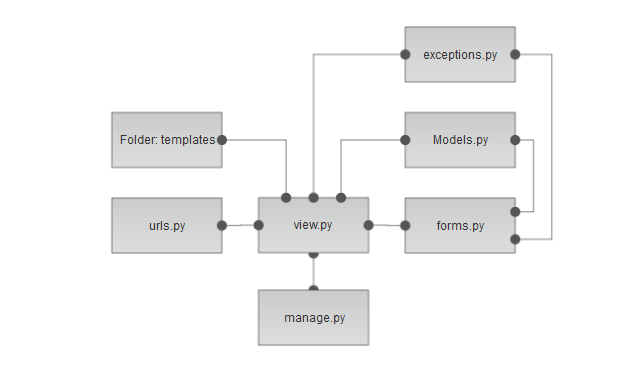
\includegraphics[width = \textwidth]{FileStruct.png}
%	\caption{Denne figur viser kommunikationen mellem filerne i projektet.}
%	\label{fig:fileStrk}
%\end{figure}
Vi har brugt introduktionen til Django til at starte vores projekt. Denne introduktion tager udgangs i en hjemmeside til at lave meningsmålinger, og derfor vil man se at vores program indeholder udtryk som mappen 'polls'. Vi har snakket om at fjerne dette, mest fordi det ser grimt ud, men har valgt ikke at gøre det, da der er meget der henviser til polls rundt om i applikationen. Ud over det lidt vildledene navn 'polls' har oprettelsen af et Djangoprojekt gennem introduktionen også gjort at vi har et hav af filer rundt omkring. Vi er ikke 100\% klar over hvilke af disse filder der bruges af Django - og derfor ikke kan slettes - og hvilke Django blot oprettede for at man kan tilføje objekter i dem. Vi har derfor valgt at lade dem blive for nu, da de jo ikke gør skade. Figur \ref{fig:fileStrk} viser sammenhængen mellem de filer vi bruger. Ud over disse filer har vi også tests.py, denne fil og dens historie, funktioner og placering på kortet kan der læses mere om i afsnit \ref{Afprovning}.

\subsection{Kodens struktur}

I filen models.py har vi lagt alle tabeller i databasen - også omtalt som clases - og deres tilhørende funktioner. Strukturen af models.py er, på samme måde som fil strukturen, sådan at de forskellige classes kun kender til hinanden hvis de har brug for det. 
%Se figur \ref{fig:database}.
%\begin{figure} [H]
%	\centering
%	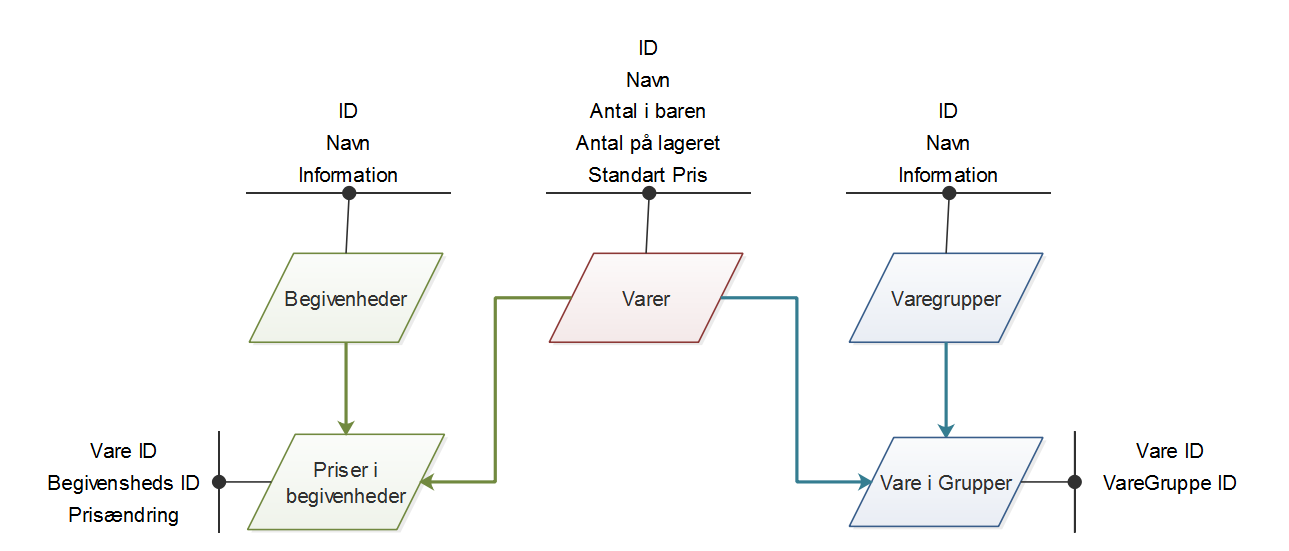
\includegraphics[width = \textwidth]{Database.png}
%	\caption{Denne figur viser kommunikationen mellem de tabeller der ligger i programmets backend.}
%	\label{fig:database}
%\end{figure}
\noindent Under hver class ligger der så en række funktioner. Disse bruges til at søge og ændre i database. Flere af disse funktioner er allerede predefineret i Django, men vi har af forskellige årsager haft behov for at ænder dem.
%\begin{wrapfigure}{r}{0.5\textwidth}
%	\vspace{-25pt}
%	\begin{center}
%		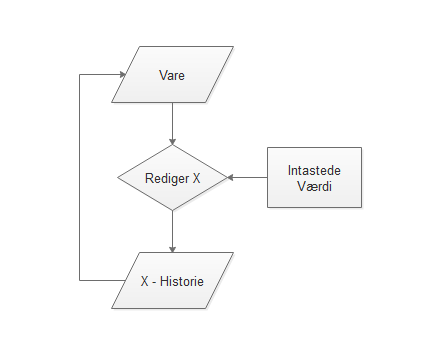
\includegraphics [width=0.48\textwidth] {ChangeValue.png}
%	\end{center}
%	\vspace{-25pt}
%	\caption{Denne figur viser den nye funktionsstruktur for at gemme en ændring i en tabel. Denne funktion er så skrevet for hver tabelværdi (substituer x med felterne i de forskellige tabeller som ses i figur \ref{fig:database}).}
%	\label{fig:Change}
%\end{wrapfigure}
\noindent Django har fx en simpel måde at gemme nye værdier i databaser. Men denne metode overskriver blot værdien, og man mister derfor historien. En af de ting der var et krav fra forbrugeren var at man kunne se historikken for fx prisen af en vare. Sådan at når man ændrede prisen, så havde denne ikke indflydelse på tidligere optællinger. Dette er løst ved at lave en tabel i databasen for hvert felt i de i figur \ref{fig:database} angivet clases. Funktionen til at redigere et felt i en tabel i databsen er så ændret til at se ud som på figur \ref{fig:Change}, sådan at enhver ændring gemmes i en særskilt tabel, med et tidsstempel og den nye værdi. En ander for vi havde i tankerne var at lave en ny tabel hver gang der blev lavet en ændring (fx en optælling). Denne skulle så have datoen og tiden for optællingen som navn, og skulle indeholde alt information som var i tabellen Vare. Vi valgte ikke at bruge denne da den ville fylde vores database med tabeller, som ville være svære at tilgå da man skulle kende tidspunktet for ændringen. Det ville blive uoverskueligt at finde ændringer, og databasen ville blive stor, og dermed kunne vi resikere hurtigt at få en ustabil database. 

\subsection{Overvejelser omkring koden}

Både Agile og CC \cite{martin2006agile,boswell2011art} forklarer fordele ved at inkapsulere koden hensigtsmæssigt samt korrekte måder at opbygge nedarvninger og interfaces. I forbindelse med dette projekt har der ikke været gjort brug af disse principper i egenproduceret kode. Det ville have været muligt at lave en modelklasse med eksempelvis historik -elementer som alle andre historikker arver fra. På samme måde er eksempelvis alle deletethis for Wares, Waregroups og Events af meget ens natur. Kodens størrelse har dog ikke givet indtrykket af at dette ville have sparet meget tid ift dette projekt, men mere haft en gavnlig effekt på korrekte vaner til fremtidige projekter. \\
\indent Der er heller ikke oprettet interfaces for Models som kan tilgås af eksempelvis Views og Forms, hvor koden på samme måde ikke virker som af en størrelse hvor dette er stærkt nødvendigt.\\
\indent Variabelnavne, funktionsnavne og klasser er ikke blevet udviklet på baggrund af en fastlagt konvention, men det er forsøgt at benytte indsigten fra CC \cite{boswell2011art} omkring navngivning af variabler. Så vidt muligt har funktionskaldende taget højde for \textit{functional cohesion} som beskrevet i \textit{code complete} 

\subsection{Design/analyse - Forholdet mellem backend og frontend}

Hvis et design skal være ordentligt modulariseret bør backend være ligeglad med hvilken frontend der anvendes. I mindre grad bør man også kunne tage en del af backend som eksempelvis wares og anvende til andre formål. Wares indeholder dog eksempelvis en funktion som "getopeningwares" der forholder sig til behovet for at registrere indeholdet for åbne varer, hvilket ikke nødvendigvis ville være relevant i et andet optællingssystem. Der er dog to indvendinger mod at skulle tage modulariseringen til den slags højder. For det første er det begrænset hvor meget ny kode der er i Wares relativt til blot at skabe et nyt djangoprojekt. For det andet kan man risikere at en sådan generalisering hurtigt kunne ende med at fjerne fokus fra slutproduktet (et funktionelt program) til fordel for designfilosofi.\\
\indent På trods af denne antagelse om hvad backend skal anvendes til er der dog ikke ellers en sammenblanding af backend og frontend. Models.py gør udelukkende brug af exceptions.py og djangos underliggende biblioteker. 
\indent Frontend er klar over backendfunktionaliteterne og disse er ikke indpakket i interface. Derudover udføres checks omkring hvorvidt baren er åben i frontend. Disse checks kunne med fordel flyttes til backend, da man ellers er i den problemstilling at et faneblad kan åbnes af een bruger mens en anden eksempelvis åbner baren. Muligheden for at redigere i oplysningerne for den første bruger vil dermed være tilstede selvom systemet ikke burde tillade det. Havde man flyttet disse checks til backend havde man yderligere besværliggjort modulariseringen men samtidigt sikret et mere hensigtsmæssigt program til den aktuelle kunde. Disse problemer kunne selvfølgeligt igen modvirkes ved at pakke kommunikationen mellem backend og frontend ind i et interface.

\subsection{Design/analyse - Priser}

Der har gennem tiden været mange overvejelser om hvordan vi skulle håndtere de forskellige priser i de forskellige begivenheder, har under har der været flere forskellige udgaver af en standard pris

\subsubsection{Uafhængige priser}
Som udgangspunkt kunne man have en pris til hver begivenhed og vare/varegruppe der var uafhængig af alle andre priser. Dette virkede dog ikke hensigtsmæssigt for kunden, da kunden dermed enten skulle have afklaret prisen for alle varer for en given begivenhed, når denne begivenhed blev oprettet, eller at kunden skulle acceptere at prisen for en bestemt vare kunne stå i 0, hvis oplysningen ikke var til stede ved oprettelsen.\\
Vi fandt det i gruppen mere hensigtsmæssigt at systemet for varen/varegruppen ville falde tilbage på en pris, hvis ikke der var angivet en pris for den givne begivenhed. Problemet blev så hvordan denne pris bedst kunne gemmes.

\subsubsection{Standardbegivenheden}
En anden overvejelse var at have én af begivenhederne til at have rollen som standardbegivenhed. Denne begivenhed ville have en pris for hver vare/varegruppe. Når en bruger ville oprette en ny begivenhed kunne systemet dermed enten hente disse priser ind til efterregulering eller bruge dem når brugeren ikke havde indtastet specielle priser. % ?? eller gøre det muligt at kopiere hele standardprisbegivenheden for så at redigere den som et separat 'objekt'.??
Den store fordel ved dette design var dets enkelthed i konstruktionen. Det er en meget intuitiv tilgang til problemet "I denne begivenhed koster denne vare dette". Men vi kunne igen se nogle uhensigtsmæssigheder for både os kunden. \\
\indent På vores side ville vi skulle have en måde at afgøre hvilken begivenhed der var standardbegivenheden. Dette kunne være den først oprettede begivenhed, men hvis kunden ønskede at slette denne eller kom til det ved et uheld, kunne der nemt ende med at være mange tilfælde, vi skulle forholde os til i koden. \\
\indent Fra kundens side ville udfordringerne i høj grad komme, når systemet havde været brugt i et stykke tid. Hvis man ændrede prisen på en vare, ville man være nødt til at gøre dette for alle begivenheder. Hvis der ikke altid var en relation mellem standardprisen for varen og begivenhedsprisen, kunne man dermed ende med et større vedligeholdelsesarbejde. 

\subsubsection{Varespecifiseret standardpris}
Den tredje designovervejelse, som vi endte med, var at sætte en standardpris for varen og derefter lade begivenhedspriserne blive bestemt i et forhold til denne pris. Hvis kaffe normalt kostede fem kroner, men man om mandagen ville give en rabat på to kroner, kunne mandagsbegivenheden haven differenceprisen for kaffe sat til -2 kroner. Kaffen ville dermed i systemet fremstå med en pris på 3 kroner om mandagen.\\
Skulle den generelle pris sættes op fra 5 til 10 kroner ville mandagsprisen dermed også stige fra 3 til 8 kroner. Den absolutte besparelse ville dermed være bevaret.

\subsubsection{Brugerflade}
I overvejelserne om brugergrænsefladen er der fremstillet to forskellige variationer af prisfastsættelsen for begivenheder. den ene bevarer den intuitive tilgang fra det første design er frontenden konstrueret sådan at den udregner total prisen for en given vare i en given begivenhed og viser denne til brugeren når man ser på listen over priser i begivenheder. Så hvis man eksempelvis slår kaffe op under begivenheden "Mandag" står der blot 3 kr. Dette betyder også at hvis man skal sætte prisen for en vare for en begivenhed vil man blive bedt om at sætte den pris der skal være for den begivenhed. For at demonstrere de forskellige mulegerheder er dette anderledes hvis man skal sætte prisen for en varegruppe for en begivenhed. Her vil man blive bedt om at notere hvor meget dyrere eller billigere varegruppen skal være for den begivenhed.  

\subsubsection{Varegruppe- eller blot varespecifiseret priser}
Vi skulle her have konfereret med kunden om hvorvidt der var et ønske om at lade varen bestemme prisen frem for varegruppen, som de har gjort indtil nu. Ønsker de at fortsætte med at lade varegrupperne angive priserne kan dette dog implementeres uden de store omkostninger.

\subsection{Design/analyse - Håndtering af sprut} \label{Sprut}

Det er nødvendigt for nogle varer at kunne håndtere særlige oplysninger. Konkret har kunden ønsket at man kan notere vægten af sprut for åbne sprutflasker. I overvejelserne omkring, hvordan denne problemstilling kunne løses kom vi frem til følgende muligheder:

\subsubsection{Underklasse}
Man kunne lade sprutflasker som en underklasse for varer m.fl. potentielle underklasser senere. Altså lave en helt ny tabel i tabellen varer. Denne mulighed blev ikke udforsket grundigt, da vi ikke var sikre på hvor nemt det var at operere sådan med objekterne, når der reelt var tale om tabeller i en database. Vi var blandt andet usikre på, om der ville være utilsigtede konsekvenser for muligheden for at kunne hente alle varer baseret på id.

\subsubsection{Ekstra felter}
Man kunne indsætte ekstra felter for alle varer. På denne måde ville det for vores vedkommende ville det blot være en ekstra værdi i tabellen. \\ 
\indent Dette virkede uhåndterbart for kunden da han så ville have et rastfelt ud fra alle varer og hvis priserne for de åbne varer skulle håndteres korrekt, kunne man nemt ende med mange ekstra oplysninger for en vare. [\cite{boswell2011art} Hvis dette skulle håndteres kunne man nemt ende med et brud på \textit{Code Completes} design-filosofi om flags.\\
\indent \textbf{Bool som redning}\\
Man kunne lave en bool for sprut som en del af oprettelsen af en vare i kombination med ovenstående. Der ville dermed kun være ekstrafelter for kunden, når disse varer talte som sprutflasker.\\
\indent Her ville problemerne dog være det samme som for forrige punkt, så dette virkede som en lappeløsning for en lappeløsning.\\
\indent \textbf{Varegruppe med særlige egenskaber}\\
Man kunne lade sprut-egenskaberne være bestemt af varegruppen. Man kunne dog dermed risikere at klasserne blev bundet for tæt sammen og de ekstra felter for vareoplysninger skulle stadig inkluderes i varen selvom de ikke var synlige for kunden. Hvordan varegruppen skulle noteres som en sprutvaregruppe og om dette var reversibelt kunne også give problemer længere henne i udviklingen.

\subsubsection{Oprettelse af (åben) varen}
Den sidste mulighed i vores designrække, som også er den vi valgte, er muligheden for at oprette en sjatvare når man opretter en ny vare i systemet. Dette har fordelen at vi ikke skal ændre i vores i forvejen eksisterende kode. Der skal blot laves en funktion der kopiere de indtastede værdier for den oprettede vare, og tilføjer " (åben)" efter navnet. Endvidere kan funktionen bede om en ny enhedspris for (åben)varen. I frontenden vil kunden kun se en tjekboks under oprettelsen af en vare, tjekkes denne af bliver kunden sendt videre til oprettelsen af (åben)varen når der trykkes gem. Når kunden tæller op vil disse vare så være lige ved siden af hinanden, både hvis der sorteres efter navn og ID. Enhederne som denne (åben)vare kan optælles i vil helt op til kunden, de skal blot indtaste den nye enhedspris. Ønsker de fx at fortsætte med at opgøre i gram skal de blot være enige om dette og skrive prisen pr gram, når (åben)varen bliver oprettede.\\
%Dette har muligvis ført til beslutningen i designstadiet for at sætte en stdpris på varen i stedet for varegruppen. Det er dog ikke nedskrevet i noterne for gruppens diskussioner.
\indent Denne løsning kræver dog ved når efter tanke (og ved hjælp af testresultater) at vi foretog en lille ændring i vores åbne/lukke funktion. Denne viser kun vare der er på lager, og man kunne så komme ud for at (åben)varen ikke ville figurere på listen ved lukning, hvis man ikke havde en åben flakse ved åbning af baren. Dette problem er løst ved at medtage vare der i navnet indeholder strengen " (åben)". Dette er en simpel metode, en bedre løsning kunne være mulig. \\
\indent Der er i øjeblikket ingen checks for, om den åbne vare allerede eksisterer ved navn og derfor ikke vil blive oprettet af systemet. Ligeledes bliver brugeren ikke gjort opmærksom på varens natur som sprutflaske, kagepakke eller hvad kunden ellers kunne ønske at opgøre i lukket og åbne varer i fremtiden. \\
\indent Generelt for overvejelserne af denne problemstilling skal det nævnes at vi følte os usikre på, hvordan kunden helst ville ønske en sådan implementering. De følgende mailkorrespondencer gjorde os dog ikke klogere på kundens ønsker, da vi havde indtrykket af, vi talte forbi hinanden. Den lurende deadline fik os dermed til at træffe en beslutning på baggrund af egen intuition, selvom et fysisk møde med kunden nok havde været mere praktisk i en normal udviklingssituation. Dette stemmer også overens med det agile princip om at arbejde fysisk sammen med en kunderepræssentant \cite{martin2006agile}.

\subsection{Design/analyse - Håndtering af vareændringer bagudvendt}

Et af de ikke trivielle behov for kunden var ønsket om at have en mulighed for at se hvad et element i databasen havde haft af oplysninger tidligere. Normalt vil et databaseelement ikke opbevare oplysninger om tidligere stadier. Samtidigt ønskede vi ikke at disse tidligere oplysninger kunne påvirke systemet i normal produktionssammenhæng.

\subsubsection{Fil med ændring}
En måde at håndtere dette på var at lade hvert element blive skrevet ud til eksempelvis en fil med alle oplysninger før og efter skrevet med tidspunkt for ændring. En sådan løsning virkede rimelig nem at implementere, men ikke særligt brugbar for fremtidig udvikling. Som en del af kravspecifikationen havde kunden ønsker om at systemet skulle kunne integreres med et regnskabssystem. En tekstbaseret udskrift ville være meget svær at udnytte til et sådant regnskab og ville kræve mange regulære udtryk som hurtigt kunne kræve meget lange køretider for at give et svar.

\subsubsection{Tabeller med ændringer}
En anden måde var at lade hvert af disse udskrifter foretages til en databasetabel i stedet. Man kunne gemme eksempelvis varens felter hver gang en ændring var foretaget. Dette ville inkludere mange uændrede data som blev kopieret, da man kunne være forholdsvist sikker på at en bruger ikke ændrede varens navn samtidig med en optælling. Der var også en bekymring for hvordan disse ekstra oplysninger kunne påvirke et fremtidigt regnskabssystem.

\subsubsection{Felt historik}
Som alternativ til forrige løsning valgte vi at oprette en historikklasse for hvert felt i tabelobjekteterne. Dette skabte mange ekstraklasser i models.py, men da deres funktionalitet indtil videre er begrænset, var de nemme at sikre til en nogenlunde tryghed over koden. Det er så meningen at disse historikker kan sammenlignes baseret på deres publiceringsdato og man dermed kan finde eksempelvis prisen for en vare for en begivenhed og gange med antallet af solgte varer for at finde indtægten en given dag.
\pagebreak[3]

\section{Afprøvning} \label{Afprovning}
I dette afsnit vil vi gennemgå de overvejelser vi har haft om forskellige tests af systemet. Afsnittet vil omhandle både backend og frontend tests. Vi vil reflektere over brugen af både de manuelle og automatiske test, samt overvejelser og brug af testfunktioner. 

\subsection{Overordnede overvejelser for afprøvning}

I forhold til den agile softwareudviklingsfilosofi er det vigtigt at tests udføres som en del af kodningen. Disse tests skal i den agile filosofi helst skabes før man laver den egentlige kode, således at man opnår en række fordele. Disse fordele inkluderer at man har dokumentation for hvordan koden virker, der ikke bliver forældet, at man tvinges til at gøre grundige overvejelser om hvad koden faktisk skal kunne og at man faktisk får lavet en række tests til at mindske antallet af fejl der kan opstå i koden.\\
\indent Der er dog en række udfordringer ved test-first, som vi har oplevet i forbindelse med  udviklingen af vores kode. Den ene udfordring blev skabt i forhold til at arbejde i et hidtil ukendt udviklingsmiljø. I forsøget på at lære teknologien at kende, kan det være fordelagtigt at modificere kode fra dokumentationsdokumenterne for at se, om man kan få noget funktionelt der i højere grad passer til egne behov. Ved denne indlæringsprocess kan man ende med fint brugbar kode, som man ikke har udviklet tests for. Dette bryder test-first mentaliteten, men giver en mere effektiv start på kodenings processen. En anden udfordring ved test-first er det brud på udviklerens \textit{flow}, som skiftet mellem tests og funktionel kode kan give. Når man er i udforskningszonen kan det føles som dobbeltarbejde hele tiden at skulle skrive en testkode. Vi har i stedet valgt at skrive koden som vi tænkte den bedst, og så skrive testscenarier i en testfunktion for at test alle de mulige scenarier vi kunne komme i tanke om. \\
\indent Den sidste udfordring har været, at ikke al kode kan testes på lige fod. De automatiserede tests blev udviklet i forbindelse med backend, men Django-dokumentationen gav ikke umiddelbart beskrivelser af, hvordan man lavede tests for view-metoder. Beskrivelserne fra dokumentatioen fokuserede på Djangos Form- og View-klasser, men disse blev benyttet i begrænset omfang i vores projekt.

\subsection{Automatiserede tests}

De automatiserede tests er sat ind i filen cafeen/tests.py. Disse tests er blevet kørt ved at benytte kommandoen 'python tests.py test'. Django har allerede leveret en tests.py fil i cafeen/polls/tests.py, men denne blev ikke benyttet til at starte med og siden har den nuværende test-fil fået lov at overleve fordi der altid har været større prioriteter i arbejdet. den anvendte tests.py har fået indsat koden fra manage.py. Dette er reelt ikke nødvendigt, men har også fået lov at overleve fordi andre dele af koden har haft større prioritet. \\
\indent De anvendte testcases er designet ud fra den filosofi at hver funktion principielt kun afdækker een funktionalitet i programmet. Med denne bagtanke er testene for hver funktion rimeligt udvidede. Frem for bare at teste een ting per test kan adskillige scenarier testet i en testfunktion, men hvor fokus i alle scenarierne er at afprøve den relevante funktion. Dermed kan der være adskillige asserts per test.
\indent De automatiserede tests dækker kun et subset af koden. Da view-funktionerne og form-klasserne blev dannet, var det ikke afklaret hvordan man overhovedet skulle teste disse klasser og funktioner, da en del af testen ville kræve en form for simuleret brugerinput og da en stor del af skabelsesprocessen for view-metoderne handlede om at afklare, hvordan Django fungerede. Da kodningen var en del af en læringsprocess virkede tests ikke oplagte. Konsekvensen var at vanen med at danne tests blev brudt og deadline for opgaven nærmede sig, så senere klasser som Openandclose i models.py har heller ikke fået oprettet automatiserede tests. \\
\indent De automatiserede tests blev udført samme dag som den respektive kode der skulle testes. Dog var det kun i nogle af tilfældende at testene blev udviklet først. De automatiserede tests viste sig gode til at opdage fejl som var en konsekvens af andre rettelser. Derudover mindskede det problemerne ved det kodegenbrug, som fandt sted ved designet af backend. Ved kopieringen af visse funktioner hændede det at den forkerte historik blev kaldt. En sådan fejl kunne nemt have sneget sig igennem systemet hvis ikke de automatiserede tests fangede problemet med det samme.

\subsection{Manuelle tests}

I de situationer, hvor der ikke blev oprettet automatiserede tests, blev softwaren testet manuelt. En af disse typer manuelle tests bestod af \textit{print()}-kald indlagt i koden for at se om kodens \textit{conditionals} blev eksekveret korrekt. Disse tests grænsede til debugging, men blev også brugt når der blot var uklarheder under læringsprocessen for Djangos funktionaliteter. En anden metode var at indtaste forskellige værdier i frontendsystemet for så at se om konsekvenserne ved indtastningerne svarede som forventet. Disse manuelle tests mindede om brugerfladetsts, men fokus var ikke nødvendigvis i brugerfladen, men derimod funktionaliteten. 
Fælles for disse metoder er, at de ikke permanent tester koden, samt at de faktisk nemt ender med at tage mere tid, end man kunne forvente fra automatiserede tests. Dog har metoderne den fordel, at de kan tvinge en til reflektion over, hvad man faktisk ønsker, at koden skal kunne og kan hjælpe med at lære en, hvordan de underliggende biblioteker fungerer. Her tænkes bla. på request.POST beskrevet under debugging.

\subsection{Brugerfladetests}

Som en del af de manuelle tests var det nødvendigt at intaste værdier gennem den udviklede brugerflade. Udover indsigten fra resultaterne ift backend-/frontend-funktionaliteten gav dette også en mulighed for at reflektere over slutbrugerens oplevelser og muligheder. Et eksempel er mulighed for at ændre i varer mens baren er åben eller hvor mange klik brugeren kan forventes at skulle udføre for at få den ønskede effekt. \\
\indent Brugerfladetesten fangede også en problemstilling i det overordnede design, der ikke var blevet overvejet tidligere eller fanget af de automatiserede tests. I forsøget på at skifte en vares associerede varegruppe, blev denne blot tilføjet en liste af associerede varegrupper. Når man skulle finde varens varegruppe, fik man dog kun det første resultat, hvilket betød at det ikke var muligt for brugeren at ændre varegruppeassociationen efter første valg. Dette tvang os til at afgøre om det overhovedet gav mening at en vare kunne tilhøre flere varegrupper. Vi har ikke haft brugerflade test af egentlige brugere. Noget der helt sikkert kunne have hjulpet på udviklingen af brugerfladen, men vores fokus har været en funktionel backend, og derfor har dette ikke være et fokus.  

\subsection{Debugging case 1}

Ved brugerinput blev de indtastede værdier i nogle situationer ikke modtaget. Tidligere havde der været problemer med Django-undtagelserne AttributeError og KeyError. Disse kom eksempelvis når kun nogle informationer var indtastet. Da disse fejl kom i starten af implementereingen af brugergrænsefladen, var views-metoderne ikke tilpas forstået endnu. For ikke at gå i stå blev disse fejl ikke rettet/fundet i første omgang. I stedet blev arbejdet med views-metoder droppet for at bevæge sig over i views-klasser og form-klasser i stedet. Da dette heller ikke gav den ønskede brugerflade, blev metoderne genanvendt med lappeløsninger på problemet, dog med et "\#TODO:" skrevet ind i koden for at markere at denne kode ikke var korrekt udformet. Relativt sent i projektet blev det opdaget ved et tilfælde at request.POST krævede en yderligere conditional end tidligere planlagt. Den manglende overvejelse skyldtes en misforståelse af, hvornår django eksekvere sin kode.

\subsection{Debugging case 2}

Implementeringen af at kunne sætte varegruppers priser baseret på en begivenhed var blandt de sidste funktionaliteter, der blev tilføjet til brugerfladen. Enkelte varer kunne allerede prisjusteres, så opgaven blev vurderet som relativt triviel. Da implementeringen blev testet endte Django dog i flere tilfælde med at give en IndexError. Det var ikke muligt at finde fejlen blot ved at følge loggen og da problemet inkluderede problemet fra case 1, blev der behov for at dykke ned i præcis hvad der skete i koden.\\
\indent Første skridt var at udkommentere en række af de kald, som view-metoden gjorde brug af, således at fejlens mulige placeringer kunne isoleres delvist. \\
\indent I andet skridt blev print-statements indsat i view-metoden ved hvert 'if' og 'else' for at kunne afgøre, om koden opførte sig som forventet. Misforståelsen fra case 1 blev fundet ved denne metode, men ellers fungerede koden som forventet. \\
\indent I tredje skridt blev View-metodens kald genindført og den kaldte form-klasse blev i stedet udsat for udkommenteringer og print()-funktioner. I stedet for at printe at koden kom til et bestemt stadie i koden var der dog her større interesse for hvilke id-værdier, som blev kaldt, da dette øjensynligt var årsagen til den fundne IndexError. Den anvendte hypotese på dette tidspunkt var, at WaresInwWregroup-relationen ikke korrekt havde slettet en relation, da en vare blev slettet. Dette kunne blandt andet være sket i testdatabasen, fordi denne ikke var blevet renset under udviklingen af funktionaliteten.  \\
\indent Blandt de givne resultater kom et vareid op der var blevet slettet tidligere på dagen. Dette virkede umiddelbart til at bekræfte hypotesen, men varen var ikke registreret i WaresInWaregroup. En kortlægning af relationerne i WaresInWaregroup viste at der her ikke var nogen fejlregistreringer. Samtidig var det muligt at se der ikke var nogen sammenhæng mellem de resultater man fik ved at tilgå WaresInWaregroup direkte og så den måde det foregik på og de resultater der kom fra form-klassen.\\
\indent Under endnu en granskning af form-klassen viste det sig, at et af variabelnavnene var forkert. En variabel var sat til ware, selvom det var en samling af Waresinwaregroup-objekter. Dette havde skabt en misforståelse senere i koden, hvilket bevirkede at ware.id ikke som forventet havde fundet varens id, men derimod den id, som Waresinwaregroup-objektet havde. Ved at ændre ware til warerelation og ware.id til warerelation.ware.id forsvandt alle uoverensstemmelserne. 

\pagebreak[3]


\section{Udviklingsmiljø} \label{Udviklingsmiljo}
% Beskriv jeres udviklingsmiljø, herunder anvendte programmeringsmiljø, opsætning af projektet i GitHub, plan for versionsstyring, mv. Forklar hvordan filer i projektet er struktureret. Forklar endvidere hvordan jeres applikation bygges og afvikles.
% Dette afsnit skal kunne læses af nye udviklere som vejledning i at sætte et udviklingsmiljø op og påbegynde videreudvikling på projektet.
% I skal endvidere diskutere, hvordan jeres udviklingsmiljø og de værktøjer I har brugt, effektivt understøtter arbejde med programmering, refaktorering, afprøvning og afvikling af applikationen.
I dette afsnit vil vi gennemgå vores udviklingsmiljø. Vi vil gennemgå opsætning af vores undeliggende teknologi, Python - Django \& SQLite - samt valget af værktøjer, PyCharm, Kate og GIT.

\subsection{Underliggende teknologi}

De underliggende teknologier benyttet i projektet har været Django som importeret modul til Python. Databasen er SQLite, selvom denne var abstraheret væk i Djangos biblioteker.  \\
\indent \textbf{Python} blev valgt af gruppen fordi det var et programmeringssprog som alle i gruppen havde et vidst kendskab til. Python kan både benyttes som et scripting-sprog og et objectorienteret sprog. Kendetegnende ved Python er det manglende behov for kompilering og den relativt svage typecheckning. Det manglende behov for kompilering muliggjorde at man hurtigt kunne køre en automatiseret test efter en ændring eller teste manuelt efter hver kodet linie. Disse muligheder blev benyttet til at raffinere koden flere steder uden at opleve ventetider \cite{martin2006agile, boswell2011art} \\
\indent \textbf{Django} blev valgt på anbefaling baseret på at det både indeholdt fleksible værktøjer til manipulation af en database og værktøjer til at konstruere hjemmesider med indbyggede sikkerheder mod blandt andet SQL-injections. Derudover gav førstehåndsintrykket os et håb om, at vi ikke behøvede at bevæge os meget ud for dokumentationen for at få svar på problemstillinger, man kunne støde på i forbindelse med brug af teknologien. Dette håb viste sig at få os til at undervurdere bestemte funktioners tidsmæssige omkostninger. \\
\indent I forhold til Djangos indbyggede funktionaliteter er særligt fem moduler blevet benyttet: Models, Forms, Views, URLs og Testscases. Derudover er Djangos templates også blevet benyttet til at generere browsersiderne. \\
\indent \textbf{Models} gjorde det muligt for os at oprette og manipulere med databasen som var det simple objekter. Inden vi opdagede denne mulighed havde vi allerede oprettet flere af de fornødne SQL-koder for at opnå den ønskede funktionalitet, men muligheden for at indkapsle disse koder med en større sikkerhed for at undgå fejl var en klar fordel for projektet. Mere komplekse SQL-kommandoer krævede brug af et særligt Q-object fra Models, men dette viste sig ikke at være en større udfordring for projektet. \\
\indent \textbf{Forms} gjorde det muligt at manipulere med Models baseret på input givet at slutbrugeren. Med denne funktionalitet stødte vi ind i en række problemer, hvilket har mindsket vores fulde udbytte af teknologien. Bl.a. ved søgning på stackoverflow viste det sig at Forms-klasser ikke er designet til at skulle indgå flere gange på samme side, hvorimod normale html-forms godt kan skrives ind i en forløkke. Derudover var det en begrænsning for udviklingen af en frontend at vi i en stor del af projektet ikke troede, at det var muligt for os at få Form-klasser til at kalde vores egne funktioner fra Models, da vi dermed ville miste vores mulighed for at udvikle begrænsninger og oprettelse af historik. \\
\indent \textbf{Views-klasserne} var påvirket af udfordringerne med forms. Derudover viste de sig mindre intuitive end View-metoder, så i den endelige kode er der benytte view-metoder i stedet. Muligheden for at kunne tilgå templates og håndtere requests var dog en stor hjælp i produktionen af en brugergrænseflade. Brugergrænsefladen bryder med nogle af designprincipperne fra \textit{Agile} og \textit{Code Complete}, men i denne del af projektforløbet blev funktionaliteten vurderet til at vægte højere. \\
\indent Djangos \textbf{URLs} håndterede hvilke sider der kunne tilgås og hvilke view-metoder disse sider skulle kalde. \\
\indent Djangos \textbf{TestCases} gjorde det nemt at udvikle automatiserede tests så snart vi i gruppen havde besluttet os for en konvention for placering af den funktionelle kode. TestCases fungerer ligesom eksempelvis Junit ved at teste asserts og returnere en liste af fejl forbundet med koden. Disse fejl kan være exceptions som den funktionelle kode har kastet eller at ens assertions ikke har givet det korrekte resultat. \\
\indent Djangos \textbf{templates} gjorde det muligt at fremvise kode fra views og forms gennem en kontekst som blev sendt fra views-metoderne. Der var en del problemer med brugen af denne teknologi, da Djangos templates benytter et hjemmestrikket sprog til at håndtere denne kontekst. En af udfordringerne var at to lister af elementer ikke kunne gennemløbes sideløbende. Man kan med templates hente første element af en liste med \textit{"liste.0"} og få en int baseret på antallet af løkkegennemgange med \textit{forloop.counter0}. Det var dog ikke muligt at hente elementer fra listen ved hjælp af \textit{forloop.counter}, da \textit{liste.forloop.counter0} ikke først ville oversætte løkken, men i stedet ses som en kommando for liste. \\
\indent Git skulle benyttes til dette kursus. Hvert gruppemedlem havde en sesperat branch til at synronisere med og kunne derfra merge med master branch. Dette var ikke uden udfordringer, hvilket bliver beskrevet i diskussionsafsnittet.

\subsection{Brug af værktøjer}
Som distribution og versioneringsværktøj har GIT været benyttet.
I vores første delaflevering lagde vi op til, at der ikke skulle standardiseres om en bestemt IDE til udvikling. Til det efterfølgende møde med instruktorerne blev det krævet at vi alle benyttede PyCharm. Det viste sig dog at PyCharm ikke understøtter skærme med høj opløsning i Linux, hvilket gjorde programmet svært at anvende. Derfor benyttede Nicolai sig af programmet Kate, der er en simpel tekstbehandler med understøttelse af en række af de værktøjer, som bliver anbefalet i \textit{code complete}. Dog manglede Nicolais IDE \textit{error detection}, \textit{interactive help}, \textit{templates} og \textit{mergetools}. Den sidste af disse værktøjer lå muligvis bag GIT-problemerne beskrevet andetsteds i rapporten.

Søren og Camilla benyttede PyCharm og havde derfor adgang til følgende værktøjer fra PyCharm:
\textbf{Merge funktion} giver et simpelt og nemt overblik når forskellige udgaver skal samles til en. \textbf{GIT forbindelse} giver nem pull og push håndtering, samt simpel håndtering af forskellige grene af projektet.

\pagebreak[3]


\section{Proces} \label{Proces} % i udviklingen}

\subsection{Er der kodet agilt?}

En stor del af pensum handler om agil udvikling, som på mange måder har vist sig at være en effektiv samling af processer til at få brugbart software produceret.

Dette afsnit vil forsøge at klarlægge hvorvidt udviklingsprocessen har overholdt ideerne for agil udvikling. Dette gøres med udgangspunkt i det agile manifest \cite{martin2006agile}.
\begin{enumerate}
    \item Release early, release often: \\
Dette punkt kan være svært at svare med sikkerhed, da tidshorisonterne for softwareprojekter kan variere meget. Fire måneders udvkling mellem hvert release ville godt kunne kvalificere som hyppigt sammenlignet med rejsekortet, men gruppens evne til at overholde kravet relativt til to-ugers iterationer har været mindre frugtbart. Dette har i høj grad været påvirket af den manglende brugerflade, som har gjort det uklart internt i gruppen om hvorvidt en funktionalitet har været fuldt implementeret. Set fra brugerens synsvinkel er backend jo sjældent et færdigt produkt.

    \item Welcome change, even late in development: \\
Vores svar fra kunden for håndtering af sprutflasker førte ikke til en ændring af vores oprindelige tanker for implementationen. Dog blev de oprindelige designovervejelser vendt som optakt til mailkorrespondancen. \\
Forandringerne har ikke været så markante, da kunden allerede havde et godt kendskab til egne behov og ikke kom med pludselige skift fra den oprindelige specifikation. Et eksempel på pludselige skift kunne dog være, at muligheden for at indsætte kommentarer ved åbning og lukning var blevet glemt i designet, selvom det var skrevet ind som et use case. Da denne fejl blev opdaget to det under en dag at have kommentarer inkluderet i både frontend, backend og historik. Vi kan dermed sige at vores system kan håndtere ændringer og tilføjelser, også senere i processen.
    \item Deliver working software frequently:\\
Et princip for Git-oploads var, at koden skulle fungere, inden man opladede til master. Derudover blev der løbende tilføjet funktionaliteter. Det var dog først i slutningen af projektet at funktionaliteten kunne ses som brugbare i en produktionssammenhæng. 
    \item Businesspeople and developers must work together daily: \\
Dette er ikke blevet overholdt, men ville heller ikke have været et realistisk krav for en konstrueret opgave. 
    \item Build projects around motivated individuals. Trust that they get the job done:\\
Igen er dette svært at tilpasse med en konstrueret opgave udenfor en forretningssammenhæng. 
    \item The most efficient communication is face to face: \\
Dette har vores gruppe ikke været god nok til at udnytte og har formentligt været en alvorlig hæmsko i udviklingen. Mailkorrespondancerne i projektet har krævet en latenstid, man aldrig ville opleve med direkte kontakt. Dog har en væsentlig årsag til disse problemer været bundet i forsøget på at udvikle projektet mens andre fag også krævede tid. Dette ville i en professionel sammenhæng svare til at medlemmerne havde for mange forskelligartede opgaver udenfor deres rolle i projektet.
    \item Working software is the primary measure of progress: \\
Dette ligger i fin tråd med beslutningen om at nedprioritere andre dele af kurset til fordel for at få systemet til at virke. Dog har vi formentligt haft et lidt for stort fokus på dette punkt i forhold til punkt 6, da hyppige møder kunne have øget motivationen til at arbejde på koden.
    \item Should promote sustainable development: \\
Med undtagelse af gruppens inaktive periode og forsøget på at få alt på sporet igen har der været et nogenlunde jævnt tempo.
    \item Have attention to good design continuosly: \\
Der har ikke været fokus på at undgå kodegenbrug i projektet. Første prioritet har været at få kode til at virke og derefter om man kunne gøre det mere hensigtsmæssigt. Hvis ikke koden blev udviklet hensigtsmæssigt i forhold til kodegenbrug er det blevet noteret til senere rettelser. Dette er tilfældet for især views og templates, selvom klasserne i forms.py også kan forventes at skulle refaktoriseres.
    \item Maximise the amount of work not done: \\
Som det bliver beskrevet i Agile-bogen stiller vi os mildt tvivlende for, om dette nødvendigvis er en god idé i alle sammenhænge. Bogen Code complete stiller sig også kritisk for denne filosofi. I den konkrete opgave gruppen blev stillet, var der flere krav end blot at have et optællingssystem. Da disse krav også skulle kunne indfries på et tidspunkt gav det mening at diskutere startdesignet med det udgangspunkt at man ville kunne bygge videre mod den fremtidige funktionalitet. Designet handlede derfor i høj grad om følgende:
    \begin{enumerate}
        \item Sikre at man ikke spændte ben for sig selv på lang bane
        \item Opdele opgaver i uafhængige underopgaver, så det var muligt for flere at arbejde uden at frygte det var til gene for andre gruppemedlemmer.
        \item Fastlægge rækkefølgen af implementeret funktionalitet ift afhængigheder og brugbarhed.
    \end{enumerate}
    \item The team should be self-organizing: \\
Dette har i høj grad været tilfældet for vores gruppe, men ikke alle konsekvenserne har nødvendigvis været positive. Eksempelvis havde gruppen ikke valgt en projektleder, hvilket i TG bliver som en sikker vej til inaktivitet, hvilket gruppen jo netop oplevede i en periode. Gruppen er der nået i mål, uden nogen styring udefra. 
    \item The team reflects and retunes regularly:\\
Som for punkt 1 er succes indenfor dette afhængigt af, hvilken målestok man sætter. Den oprindelige rollefordeling viste sig uhensigtsmæssig grundet dens høje busfaktor, men håndteringen af Mohammeds forsvinden samt rollen for testskrivning, brugeradfærd mm. var reflektioner som der endte med ikke at være tid til at indstille sig efter. Havde der været yderligere arbejde for at få regnskabssystemet til at virke ville dette naturligvis have årsag til at arbejde med ændret rollefordeling.
\end{enumerate}

\subsubsection{Konklussion:}
Taget i betragtning hvor kort tidsfristen for projektet har været har gruppen som helhed formået at overholde flere af de principper for agil udvikling, som bliver fremhævet i manifestet. Blandt de punkter, som gruppen ikke har været gode til at overholde, er nogle baseret på manifestets fokus på egentlig virksomhedsproduktion og ikke et førsteårsprojekt .

\subsection{Kundekontakt}

I løbet af projektet blev der sendt følgende mails til kunden efter den oprindelige afklaring af kundens behov, se Bilag \ref{Mails}. I afsnit \ref{Diskussion} og ved relevante problemstillinger, vil gruppens håndtering og tolkning af disse svar blive beskrevet samt sammenstillet med det endelige produkt. \\
Til dette punkt ville det, som tidligere nævnt, have været ønskeligt at vi havde haft en fysisk kontakt med kunden. Både i forhold til afklaring af funktioner, og i form af egentlige bruger test.

\subsection{Gruppearbejde kronologi}

\subsubsection{Process op til D1}
Gruppen fik lavet en designskitse, udviklet user cases og user stories og fik dannet en idé om, hvor meget der kunne nåes på den tid, som projektet varede. Gruppen designede med henblik på at opgaven kunne deles op i mindre delområder, så vi bedst muligt undgik dobbeltarbejde.

\subsubsection{Feedback for D1}
Efter aflevering af D1 var gruppen til møde med instruktorerne. Vi blev rost for vores fremgang, men fik en række råd/stillet krav til fremtidigt arbejde.
\begin{itemize}
    \item Vi skulle arbejde med seperate Git-branches og merge disse for at få en korrekt forståelse for arbejde med Git.
    \item Vi skulle fortsætte med grafer og diagrammer som visuel vejledning i vores delafleveringer.
    \item Vores user stories var velpriorterede og veludformede.
    \item Vi blev mindet om at det var vigtigt at skrive programmeringstimer ind for hvert sprint samt at dette skulle inkludere hvorvidt arbejdet havde været for 'need to have' eller 'nice to have'-funktionaliteter.
    \item Vi bedt om at lave mødereferater for de møder, vi holdte. Disse skulle have fokus på hvad vi nåede/ikke nåede, samt hvorfor dette var tilfældet. 
    \item Vi blev også opfordret til at skrive ideer og mails til Jenny ind i delafleveringer, så det kunne noteres i vores fremgang. 
    \item Til sidst blev vi krævet at alle medlemmer af gruppen skulle bruge PyCharm. 
\end{itemize}

\subsubsection{Arbejde omkring påske}
Alle medlemmer i gruppen havde afleveringer i vores respektive andre fag til efter påske. Kombineret med lukkedage og sygdom blev gruppens muligheder for at arbejde på projektet mindsket kraftigt. Mødet efter påskeferien blev dermed primært brugt på at indhente arbejde på D2, samt kort oprids af den begrænsede fremgang. Der blev ikke aftalt en konvention for placering af funktioner i forhold til Djangos struktur, så det var endnu ikke muligt at lave meningsfulde automatiserede tests og delingen på Git var dermed også rodet. Mødet blev også påvirket af Nicolais første Git-problem, se figur \ref{fig:GitProblem}. Git-problemerne var formentligt en konsekvens af ikke at bruge PyCharm, hvilket gjorde merge mere besværligt. 
%\begin{figure} [H]
%    \centering
%    \includegraphics [width=0.8\textwidth] {GitProblem.png}
%    \caption{Denne figur viser Nicolais problemer med Git, man kan se at Git har tilføjet en af PyCharm forståelig kode.}
%    \label{fig:GitProblem}
%\end{figure}

\subsubsection{Arbejde omkring 'blok 3'-eksamener}
Ligesom påsken var ugerne lige før og under eksamensperioden for blok 3 præget af et begrænset fokus på softwareudvikling. Det var ikke muligt at samle gruppen til et fællesmøde men blev i stedet delt op i enkelt og pararbejde. En konvention for kodeplacering endte med at blive besluttet ad-hoc.

\subsubsection{Arbejde i blok 4}
Den lange dødvandsperiode for gruppen havde opbrudt rytmen for gruppearbejdet. Forsøg på at etablere en rytme igen blev hæmmet af Mohammeds manglende svar på mailkorrespondencerne, da alle andre medlemmer af gruppen dermed ventede for længe på bekræftelser. Konsekvensen var, at Nicolai endte med at tage en spurt i udviklingen af koden udenfor gruppebeslutninger. De næste par møder var præget af også at få nået delafleveringer. Erfaringer med kodeopbygnng blev derfor kun gennemgået på et overordnet plan. \\
\indent Det blev droppet at få Mohammed til at komme tilbage til gruppen. Arbejdet på at integrere en frontend med den nu udviklede backend, skulle dermed genskabes på ny, da Mohammed ikke havde lagt sin fremgang med brugerfladen op på Git. \\
\indent Gruppemøder handlede om dels at få etableret et fornuftigt design for varepriser, en diskussion over implementeringen af historik og hvordan vi kunne skabe en fornuftig frontend. \\
\indent Gruppens arbejdsperiode omkring påske samt Mohammeds forsvinden gjorde det nødvendigt at omprioritere arbejdet. Arbejdet på fagets ikke-obligatoriske aktiviteter blev kraftigt neddroslet og forsøget på at få en brugerflade til at køre blev opprioriteret. Djangos struktur viste sig ikke at passe fuldt ud til vores behov, så denne process krævede en del ny indlæring af bagvedliggende struktur. Dette førte til noget ikke fuldt ud funktionel kode, der dermed ikke blev delt på Git med det samme.
Denne manglende synkronisering førte til det andet Git-problem for Nicolai, med et tab af 200-500 linier kdoe. Problemer med at merge med Git gjorde at Nicolai lavede en backup inden han så kørte en \textit{clean}. Denne rengøring søgte dog hele computeren igennem, og slettede dermed også backuppen.
\pagebreak[3]


\section{Diskussion} \label{Diskussion} % af projektarbejde}
Dette afsnit kan opfattes som det opfølgende afsnit. Her vil vi gennemgå de sidste faktorer i projektet, og samle op på tidligere gennemgået punkter i arbejdet. 

\subsection{Manglende gruppemedlem}

I begyndelsen af projektet talte vi (gruppemedlemmerne) om, hvilke roller vi hver ville påtage os i løbet af projektet. Det lød som om, Mohammed havde godt styr på frontend, og det var noget, han ville tage sig af. Da vi nåede påske hørte vi ikke længere fra ham, og selvom vi (de resterende gruppemedlemmer) har prøvet at kontakte ham, har vi ikke fået svar. Derfor har vores arbejde med frontenden været et hængeparti i lang tid, og vi er ikke nået så langt med frontenden, som vi gerne ville og planlagde fra starten. Dette har i en periode også givet en lidt lad attitude når det kommer til gruppearbejde, da det har virket demotiverende, når der ikke har været klare linjer. Siden da har vi forsøgt at indhente den manglende frontend og arbejde for 4. \\
Vi har pr. dags dato (\today) stadig ikke hørt fra Mohammed, selvom vi stadig har været interesserede i at have ham med i processen. Vi har derfor fortsat sendt mails til ham, og skrevet ham på som en del af gruppen til ønsket rapportens forsvars dato, men ikke skrevet ham på denne rapport.

\subsection{Manglende brug af undervisning}

\textbf{D1} Efter at have afleveret den første delaflevering, D1, forholdsvist tidligt i projektets udvikling, blev alle grupperne bedt om at komme til et møde med instruktorerne, hvor vi ville få feedback af instruktorerne. Dette møde lå uden for kursets blokstruktur, hvilket gjorde det svært for vores gruppemedlemmer at møde op, da det betød, at vi var tvunget til at fravælge dette møde eller undervisning i det sideløbende kursus. \\
\indent Til dette møde oplevede de fremmødte gruppemedlemmer (Camilla, Mohammed og Nicolai)  at vi af instruktorerne fik meget negativ og personlig feedback, som blev formidlet og formuleret meget hårdt. Vi havde oplevet noget tilsvarende i løbet af undervisningen (dog i mindre grad end til mødet), men vi oplevede at det var noget, der gentog sig. Dette har betydet, at vi mistede lysten til at møde op til undervisningen og mistede lysten til at have kontakt til de tilknyttede instruktorer. Dette har medvirket, at vi i gruppen har arbejdet meget selvstændigt under projektet, og har brugt meget tid på at reflektere over egen indsats, da vi af åbenlyse grunde ikke har fået løbende feedback.\\
\indent Ovenstående har derudover medført, at det i en periode var svært at finde ud af, hvornår gruppen skulle mødes, da ingen af os ville møde op til undervisning. Dette var især et problem, da det var noget, vi først sent begyndte at tale om i gruppen, da vi hver især havde tænkt, at det måske kun var det enkelte gruppemedlem, der følte sådan. \\
\textbf{D1} Den anden aflevering, D2, lå i påskeferien, hvilket gjorde det svært for gruppen at koordinere, hvornår vi skulle mødes, og vi var internt ikke så gode til at svare på mails, da der blev holdt fri i anledning af påsken. Dette medvirkede af denne delaflevering blev afleveret for sent. \\
\indent Til den anden delaflevering sendte instruktorerne fælles holdfeedback, altså fælles feedback til alle grupper, der skriver projekt om de sociale foreninger (det er i hvert fald det vi kan læse ud af den besked, der er skrevet på Absalon). Gruppen læste denne igennem, og stillede sig undrende over for visse punkter men tog andre punkter til sig. \\
%Gruppen har ikke modtaget feedback eller undervisning siden den feedback, vi fik på den anden delaflevering, som ikke nødvendigvis var rettet mod gruppen, da der var tale om fælles holdfeedback. \\
\textbf{D3} Vi fik feedback på den tredje delaflevering d. 1. juni, altså mere end en måned senere end delafleveringen havde afleveringsfrist. At feedbacken kom sent, viste sig ikke at gøre en forskel, da vi fra instruktorerne fik kommentaren "fint".\\
\textbf{D4} Den feedback gruppen fik på fjerde delaflevering har heller ikke vist sig at være særligt brugbar, da vi først fik kommentaren "ikke særlig imponerende". I gruppen var vi klar over, at denne delaflevering havde mangler, da vi i stedet var begyndt at fokusere på slutspurten, men følte dog at vi stadig gerne ville have pointers så vi vidste mere om hvor vi havde sparede for meget. Derfor sendte vi en mail til Alexander, se bilag \ref{Mails}. Dette resulterede ikke i et svar men en opdatering af feedbacken.

\subsection{Reviews} \label{Reviews}

\textbf{R1}Vi har lavet og fået ét review i denne gruppe, og dette var det første, R1.  Vi var blevet sat til at lave review på en anden gruppes delaflevering. Den gruppe, vi var sat sammen med, havde ikke skrevet meget i deres første delaflevering, D1, da de havde set deadlinen for aflevering  i sidste øjeblik, hvilket gjorde at vores review af deres D1 ikke var så dybdegående. På samme måde var deres review af vores første delaflevering, ikke særlig uddybende, da de følte vores arbejde var overvældende ifht deres. Vi har heller ikke fået dette review skriftligt, men kun en mundtlig overlevering. \\
\textbf{R2} Review af den anden delaflevering skulle have fundet sted d. 4. april, men da instruktorerne ikke kunne være til stede den dag, skrev de, at de ville rykke undervisningen fra denne dag til en anden. Den nye dato blev, d. 7. april, sat til mandag d. 11. april, hvilket var i eksamensugen for blok 3. Grundet gruppemedlemmernes eksaminer i andre kurser og korte tidsfrister fra instruktorerne lige op til eksamensugen, tog gruppen ikke del i at lave eller modtage review af anden delaflevering. \\
\textbf{R3 \& R4} Efterfølgende har gruppen af flere årsager ikke deltaget i holdundervisningen, og derfor har gruppen heller ikke fået eller givet review af delaflevering 3 og 4.

\subsection{Fordeling af opgaver i gruppen}




Vores gruppe blev dannet til første holdundervisning, hvor vi fandt sammen ved, at ingen af os kendte nogen, og at ingen af os er førsteårsstuderende. Vores gruppe blev dannet af 2 dataloger (Nicolai og Mohammed) og 2 fysikere (Camilla og Søren), og allerede da vi dannede gruppen, talte vi om forventninger til, hvor meget vi hver især forventede at kode, hvor vi også talte meget om de enkelte gruppemedlemmers kodeerfaring. \\
Alle gruppemedlemmerne forventede at kode noget, men det var tydeligt, at det var datalogerne, der havde den største interesse i at kode, og at fysikerne havde det fint med at kode lidt, men skrive mest på delafleveringerne og den endelige rapport. \\
Efter denne klarlægning blev følgende opdaling lavet:
\begin{itemize}
    \item Nicolai skulle have backend som primært ansvar.
    \item Mohammed skulle have frontend som primært ansvar.
    \item Søren skulle have overblik over begge områder og sikre at vi ikke afveg for meget fra designet. 
    \item Camilla skulle have kundekontakt og rapportskrivning som primært ansvar. 
\end{itemize}
De primære ansvarsopgaver blev uddelt i forbindelse med dannelsen af en arbejdskontrakt, hvor vi diskuterede styrker og svagheder vi havde hver især. Ansvarsopgaverne havde ikke til formål at begrænse biddrag hos en andens ansvarsområde, men blot sikre at hvert medlem i gruppen kunne få lov til at fokusere på det givne område. \\ 
\indent Fra omkring påsken, altså fra omkring tidspunktet af anden delafleverings afleveringsfrist, har vi været 1 datalog (Nicolai) og 2 fysikere (Camilla og Søren). Det tog dog de 3 tilbageværende gruppemedlemmer lang tid at indse, at Mohammed ikke svarede på beskeder og ikke dukkede op til aftalte mødetider, hvilket er en stor del af grunden til, at kodeprocessen gik meget langsomt i denne periode. Såfremt resten af gruppen havde vidst, at Mohammed ikke ville dukke op og deltage i processen, kunne vi have taget over, og vi kunne have sænket vores forventninger til, hvad vi ville kunne nå i løbet af projektet. \\
\indent Opgavefordelingen (kode/skrivning) har altså ikke været til gene for nogen, men derimod var opgavefordelingen noget vi havde aftalt fra start, og der har generelt været en meget god stemning i gruppen.

\subsection{Mailkorrespondance med kunden}

I løbet af projektet har gruppen været i kontakt med kunden (se Bilag \ref{Mails}), når vi har haft spørgsmål til, hvordan vi bedst muligt kunne løse en af de opgaver, der blev beskrevet i kravene, og når vi ikke har kunne finde et svar i vores noter, som blev taget til det indledende møde. \\
Da det er Jenny, der er repræsentant for vores kunde, Caféen?, er det hende, vi har sendt mails til, når vi har haft spørgsmål.\\
Mailkorrespondancen har generalt set været tilfredsstillende for gruppen. Vi har dog undervejs haft nogle problemer med kommunikationen med Jenny, men dette har fået gruppen til at tænke grundigt over den skriftlige kommunikation. Vi har undervejs i projektet været meget opmærksomme på den skriftlige kommunikation og været opmærksomme på, at vi skulle udtrykke klart og tydeligt, så der ikke opstod misforståelser, og så vi og Caféen?s repræsentant ikke skulle bruge unødig tid på at udrede eventuelle misforståelser. \\
Til sidst i projektet havde vi dog problemer med mailkorrespondancen, hvilket kan skyldes uklar kommunikation fra gruppens side, selvom vi tænkte meget over vores skriftlige formuleringer, og gjorde det så præcist som vi mente var muligt, men det kan også skyldes, at kunden har haft travlt og muligvis ikke har haft tid til at sætte sig dybere ind i problemstillingen. Denne tidsmangel kan skyldes, at der i denne periode har været afholdt DIKU revy.
%\subsection{Frontend}
\subsection{Git}
Fra den resterende gruppe erfarede, at Mohammed ikke længere deltog i gruppemøder, besvarede mails eller lavede kode, blev vi alle bekymrede over Git, da vores repository er oprettet med Mohammeds bruger. \\
\indent Inden afleveringen af projektet er vores repository clonede over i et nyt "ProjectCafeenC6", som nu står i Søren Nissens navn (SNissen).\\
\indent I løbet af projektet, har gruppen haft problemer med at bruge git. Vi har blandt andet oplevet, ikke at kunne committe, push'e og pull'e, men det største problem har været, at vi flere gange har oplevet, at git har slettet commits, hvilket har været et stort problem for gruppen, da der er mistet flere dages arbejde, som sidenhen skulle indhentes og det har medvirket, at der har været en frygt for at benytte git, og det har til tider været svært i gruppen, at finde ud af, hvor langt vi var kommet.
%Hvornår skete det?
%Store problemer med git, git sletter, og vi har derfor ikke rigtigt turde bruge det (+ på et kritisk stadie af udviklingen) + Mohammed 
\subsection{Krav}
Den oprindelige liste af 13 krav, som gruppen formulerede på baggrund af kravspecifikationen er blevet overholdt og kravene er taget i betragtning ved væsentlige beslutninger under udviklingen. Dog er punkt 13 kun begrænset overholdt grundet en overseelse sent i forløbet. Hvis to brugere åbner samtidigt vil der godt kunne blive vareoptalt begge gange. Dette vil dog være muligt at se i systemet senere og kan rettes ved at flytte de fornødne checks ned i backend. De mere vage krav under nr. 1, 3, 4 og 12 er også taget med i betragtning, således at der ikke er forsøgt at tilføje funktionalitet som kunden ikke har givet udtryk for at kunne ønske og da brugerfladen er holdt på et meget simpelt plan. I forhold til brugerfladen ville en videre udvikling dog kræve brugertests for ikke at gøre sig for mange antagelser. \\ 
\indent På baggrund af de 13 krav fra kravspecifikationen udformede vi 21 user stories. Disse blev prioriteret efter brugbarhed for kunden samt forventede afhængigheder i koden. Af disse 21 user stories forventede vi at kunne implementere de første 14 i løbet af kurset. De første 15 af disse user stories er implementeret. Det samme er user story nr. 20. Derudover er flere mere eller mindre identiske user stories også implementeret. Det at tilføje en vare er eksempelvis meget lig at tilføje en begivenhed og derfor er den ikke senere tilføjet til listen. \\ 
\indent Blandt de resterende user stories er kun tre af dem decideret ikke implementeret. Det er ikke muligt at identificere optælleren, selvom en del af backendkoden nu er udviklet. Det er ikke muligt at merge varer direkte, selvom man kan flytte varerantal fra een vare til en anden og derefter slette varen. Det er til sidst ikke muligt at printe grafer ud over prisudviklinger. De sidste to af disse user stories er dog også potentielt indbefattet af kategorien \textit{fancy features}, hvilket vi ikke havde afgjort i startfasen af designet. \\ 
\indent De sidste user stories kan siges at være delvist implementeret. Det er muligt for en kasserer at opholde regnskaber mod hinanden, men dette skal ske manuelt. Systemet er udviklet med henblik på at automatisere denne proces, men disse funktionaliteter kræver menneskelig indblanden på nuværende stadie. Derudover kan mange brugere ændre oplysninger samtidigt, men i bestemte situationer er koden ikke helt hensigtsmæssigt opbygget endnu. 
\subsection{Parprogrammering}
\subsubsection{Ordinært forløb}
Under det ordinære forløb var blev der ikke gjort brug af parprogrammering, men der blev kodning blev diskuteret. Parprogrammeringen kunne have sørget for, at vi under det ordinære forløb havde fanget fejl og havde haft en større overblik over koden løbende. \\
\subsubsection{Reeksamen}
Af gode grunde har der ikke været mulighed for parprogrammering under det korte sommerforløb, da jeg har været alene tilbage i gruppen. Parprogrammering ville have givet samme fordele som under det ordinære forløb, som er beskrevet i BOG.
\subsection{Inspektion}
Vi burde under forløbet have foretaget minimum en inspektion som beskrevet i CC. Denne inspektion kunne have fungeret som et udvidet review, og kunne have hjulpet os til at forbedre vores projekt. Denne inspektion kunne have foregået ved at hente hjælp fra en anden gruppe, udefrastående, en instruktor eller Jenny fra Caféen?.
\subsection{Korte iterationer}
Til det korte sommerforløb har der været tilsvarende korte iterationer, da jeg har haft 3 uger at gøre godt med. Dette har betydet, at ting så som at finde en "velocity" hvormed jeg kunne nå at implementere use cases ikke har været mulig og med det relativt lille antal iterationer ikke har været brugbart.

%\subsection{Teknikker}
%Hvilken feedback/teknikker/værktøjer har vi brugt, og hvorfor/hvorfor ikke?
%\begin{itemize}
 %   \item Brug af Django
%\end{itemize}
\pagebreak[3]
\bibliographystyle{unsrt}
\bibliography{Bibliography}
\newpage  % \pagebreak[2]
\thispagestyle{empty}
\section*{Bilag}
\appendix
\section{Oversigt over delafleveringer}
%\subfile{Delafleveringer}
\section{GitHub-oversigt}
https://github.com/SNissen/ProjectCafeenC6 \\
\textbf{Installationsoversigt:}
\begin{enumerate}
    \item Download zip-fil enten fra github eller den vedlagte fil
    \item Installer python 3
    \item Importer django til python 3
    \item cd til /cafeen/
    \item Kør fra mappen: 'python manage.py runserver'
    \item Åben følgende side: 'http://127.0.0.1:8000/polls/'
\end{enumerate}
    
\section{Reviews}
Ikke relevant. Beskrevet i afsnit \ref{Reviews}
%\newpage
%\includepdf[pages=-]{LogbogD4.pdf}
\newpage
\section{Mailkorrespondance} \label{Mails}
%\subfile{Mail_AppendixD4}
%\includepdf[pages=-]{InstruktMail.pdf}
%\fancyhdr{Caféen?}
%\includepdf[pages=-]{Mail_AppendixD4.pdf}
\end{document}